\documentclass[11pt,a4paper]{article}

% ------------------------------------------------
% CONFIGURACIÓN GENERAL
% ------------------------------------------------

\usepackage[margin=2.5cm]{geometry}
\usepackage[spanish]{babel}
\usepackage[utf8]{inputenc}
\usepackage[T1]{fontenc}

% Arial
\usepackage{helvet}
\renewcommand{\familydefault}{\sfdefault}

% Justificación
\usepackage{ragged2e}
\justifying

% Interlineado 1.5
\usepackage{setspace}
\onehalfspacing

% Matemáticas y tablas
\usepackage{amsmath, amssymb}
\usepackage{booktabs}
\usepackage{array}

% Imágenes
\usepackage{graphicx}
\usepackage{float}

% Ruta de imágenes
\graphicspath{{imgs/}}

% Tablas
\addto\captionsspanish{
    \renewcommand{\tablename}{Tabla}
    \renewcommand{\figurename}{Figura}
}
\usepackage[table]{xcolor}

% Hipervínculos
\usepackage[colorlinks=true,
            linkcolor=blue,
            urlcolor=blue,
            citecolor=blue]{hyperref}

% Sangría y espaciado
\setlength{\parindent}{0pt}
\setlength{\parskip}{0.6em}

% ------------------------------------------------
% DOCUMENTO
% ------------------------------------------------

\begin{document}

% ------------------------------------------------
% TÍTULO
% ------------------------------------------------

\begin{center}
    {\Large \textbf{Actividad 2: Trabajando con redes neuronales y deep learning}}\\[0.5cm]
    
    David Vicente Moya\\
    Técnicas de Inteligencia Artificial\\
    22/05/2026
\end{center}

\vspace{1cm}

% ------------------------------------------------
% REGRESIÓN
% ------------------------------------------------

\section*{Parte 1: Regresión}
\subsection*{1. Descripción de la fuente de datos}
El dataset utilizado en esta parte de la actividad es IMDb dataset of top 1000 
movies and tv shows, que contiene información relevante al top 1000 películas y 
programas de televisión según IMDb. Este dataset incluye variables como el título, el 
año de lanzamiento, la duración, el género, la calificación de IMDb, el número de votos 
y la sinopsis. El problema planteado es la predicción de la recaudación de una 
película/serie de TV.

Esta base de datos ha sido obtenida de la plataforma \href{https://www.kaggle.com/datas
ets/harshitshankhdhar/imdb-dataset-of-top-1000-movies-and-tv-shows?resource=download}
{Kaggle}, que ha su vez ha recopilado datos de la propia plataforma de IMDb. Esta base 
de datos es de uso libre bajo la licencia de Creative Commons.

\subsection*{2. Caracterización del dataset}

La variables objetivo para la regresión es \texttt{Gross}, que compone la recaudación
de la pellícula/serie de TV. Las variables de entrada que vamos a utilizar se 
corresponden con las variables con valores contínuos y los géneros de la película/serie 
de TV. \texttt{Genre} será codificado mediante one-hot encoding para su posterior uso
en los modelos de regresión.

\begin{table}[H]
\centering
\small
\rowcolors{2}{gray!12}{white}
\begin{tabular}{p{3.5cm} p{2cm} p{8cm}}
\toprule
\textbf{Variable} & \textbf{Type} & \textbf{Descripción} \\
\midrule

\texttt{Released\_Year} & float64 & Año de lanzamiento de la película (puede contener valores faltantes, por eso está como float) \\

\texttt{Runtime} & int64 & Duración de la película en minutos \\

\texttt{Genre} & object & Género(s) de la película; puede contener múltiples categorías por película \\

\texttt{IMDB\_Rating} & float64 & Puntuación otorgada por usuarios en IMDb \\

\texttt{Meta\_score} & float64 & Puntuación media de críticas profesionales (Metacritic) \\

\texttt{No\_of\_Votes} & int64 & Número total de votos recibidos en IMDb \\

\bottomrule
\end{tabular}
\caption{Variables de entrada con tipo y descripción del dataset de IMDb.}
\label{tab:variables_tipos}
\end{table}

\break

Para la resolución del problema planteado, predicción de la recaudación de una película
/serie de TV, se ha planteado su resolución con un modelo de regresión basado en redes
neuronales y otro utilizando Random Forest.

\subsection*{3. Resultados}

\begin{table}[H]
\centering
\begin{tabular}{lccc}
\toprule
\textbf{Modelo} & \textbf{MAE} & \textbf{RMSE} & \textbf{R$^2$} \\
\midrule

Red Neuronal & $6.11 \times 10^{7}$ & $9.50 \times 10^{7}$ & 0.307 \\
Random Forest & $4.32 \times 10^{7}$ & $6.98 \times 10^{7}$ & 0.626 \\

\bottomrule
\end{tabular}
\caption{Comparación de métricas de rendimiento entre los modelos de regresión.}
\label{tab:modelos}
\end{table}

\begin{figure}[H]
    \centering
    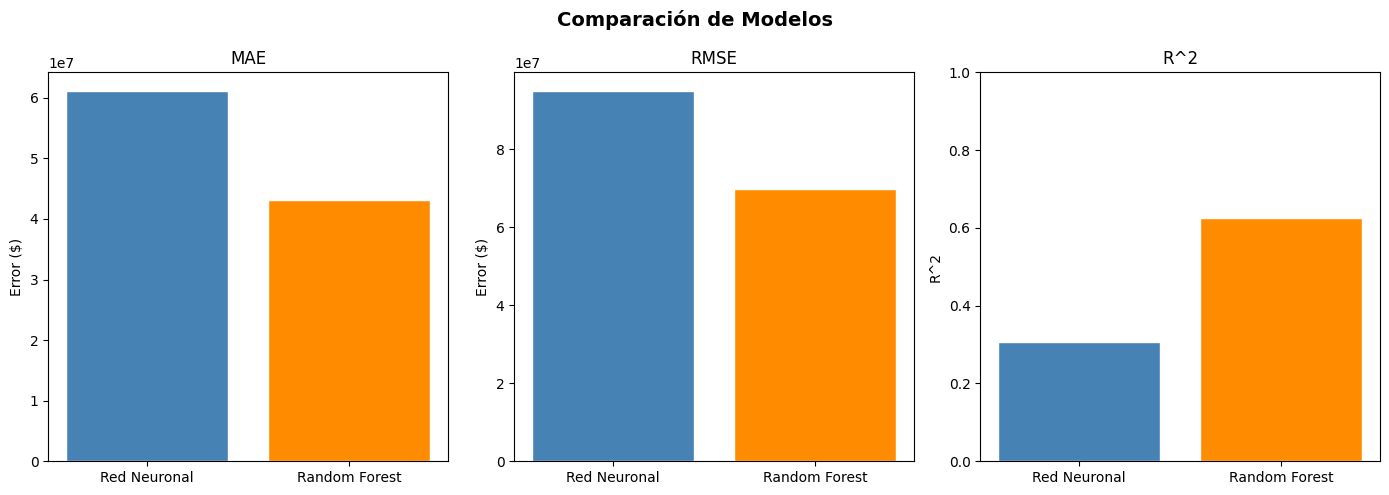
\includegraphics[width=\textwidth]{comparacion_regresion.png}
    \caption{Comparación de los modelos de regresión.}
    \label{fig:comparacion_regresion}
\end{figure}

\subsection*{4. Discusión y conclusiones}

La Figura~\ref{fig:comparacion_regresion} muestra que el Random Forest supera 
a la Red Neuronal en todas las métricas evaluadas, con menor MAE y RMSE, lo 
que indica predicciones más precisas y robustas ante valores extremos.

Además, obtiene un mejor ajuste con un $R^2$ de 0.626 frente a 0.307, explicando una 
mayor parte de la variabilidad de la recaudación. Esto sugiere una mejor capacidad de 
generalización en este dataset, probablemente debido a su tamaño reducido.

Para mejorar la red neuronal, sería recomendable aumentar el tamaño del dataset 
(además de uun mejor muestreo de los datos), aplicar transformación logarítmica sobre 
\texttt{Gross} y utilizar técnicas como Early Stopping para reducir el sobreajuste.

% ------------------------------------------------
% CLASIFICACIÓN
% ------------------------------------------------

\section*{Parte 2: Clasificación}
\subsection*{1. Descripción de la fuente de datos}
El dataset que vamos a utilizar contiene datos recogidos de varios tipos de judías. 
Estos datos se corresponden con las características físicas de la planta como la 
longitud de la vaina o la circunferencia de la judía. Este dataset pertenece a la 
Universidad Californiana de Irvine (UCI) como parte de su Machine Learning Repository, 
y se encuentra bajo licencia de Creative Commons. El problema planteado es la 
clasificacion de las judías en función de sus características físicas.

\subsection*{2. Caracterización del dataset}


\begin{table}[H]
\centering
\small
\rowcolors{2}{gray!10}{white}

\begin{tabular}{p{3.5cm} p{2cm} p{8cm}}
\toprule
\textbf{Variable} & \textbf{Type} & \textbf{Descripción} \\
\midrule

\texttt{Area} & int64 & Área de la zona del judía; número de píxeles dentro de sus límites \\
\texttt{Perimeter} & float64 & Perímetro del judía; longitud total de su borde \\
\texttt{MajorAxisLength} & float64 & Longitud del eje mayor; distancia entre los extremos de la línea más larga del objeto \\
\texttt{MinorAxisLength} & float64 & Longitud del eje menor; eje perpendicular al eje principal del objeto \\
\texttt{AspectRatio} & float64 & Relación entre la longitud del eje mayor y el eje menor \\
\texttt{Eccentricity} & float64 & Excentricidad de la elipse equivalente al objeto \\
\texttt{ConvexArea} & int64 & Área del envolvente convexo mínimo que contiene el objeto \\
\texttt{EquivDiameter} & float64 & Diámetro de un círculo con el mismo área que el objeto \\
\texttt{Extent} & float64 & Proporción entre el área del objeto y su rectángulo delimitador \\
\texttt{Solidity} & float64 & Relación entre el área del objeto y su envoltura convexa \\
\texttt{Roundness} & float64 & Medida de redondez calculada como $(4\pi A)/(P^2)$ \\
\texttt{Compactness} & float64 & Medida de cuán compacto o circular es el objeto \\
\texttt{ShapeFactor1} & float64 & Factor geométrico derivado de la relación entre área y forma \\
\texttt{ShapeFactor2} & float64 & Medida adicional basada en la distribución espacial del objeto \\
\texttt{ShapeFactor3} & float64 & Indicador relacionado con la complejidad de la forma \\
\texttt{ShapeFactor4} & float64 & Medida complementaria de propiedades geométricas del objeto \\

\bottomrule
\end{tabular}

\caption{Variables de entrada con tipo y descripción del dataset de Dry Bean.}
\label{tab:drybean_variables}
\end{table}

La variable objetivo es \texttt{Class}, la cual contiene el tipo de judía. En este 
dataset se pueden emplear todas las variables como variables de entrada sin modificación
alguna. El cunjunto de variables correspondientes a las variables de entrada se muestra 
en la Tabla~\ref{tab:drybean_variables}.

Al igual que en el apartado de regresión, se han empleado dos modelos de clasificación; 
el primer modelo basado en redes neuronales y el segundo utilizando Random Forest 
(en concreto la versión Random Forest Regressor de sklearn).

\subsection*{3. Resultados}

\begin{table}[H]
\centering
\begin{tabular}{lccc}
\toprule
\textbf{Modelo} & \textbf{Accuracy} & \textbf{F1 Macro} & \textbf{F1 Weighted} \\
\midrule

Red Neuronal & 0.919574 & 0.931687 & 0.919503 \\
Random Forest & 0.919941 & 0.931608 & 0.919981 \\

\bottomrule
\end{tabular}
\caption{Comparación de métricas de rendimiento entre los modelos de clasificación.}
\label{tab:modelos_clasificacion}
\end{table}

\begin{figure}[H]
    \centering
    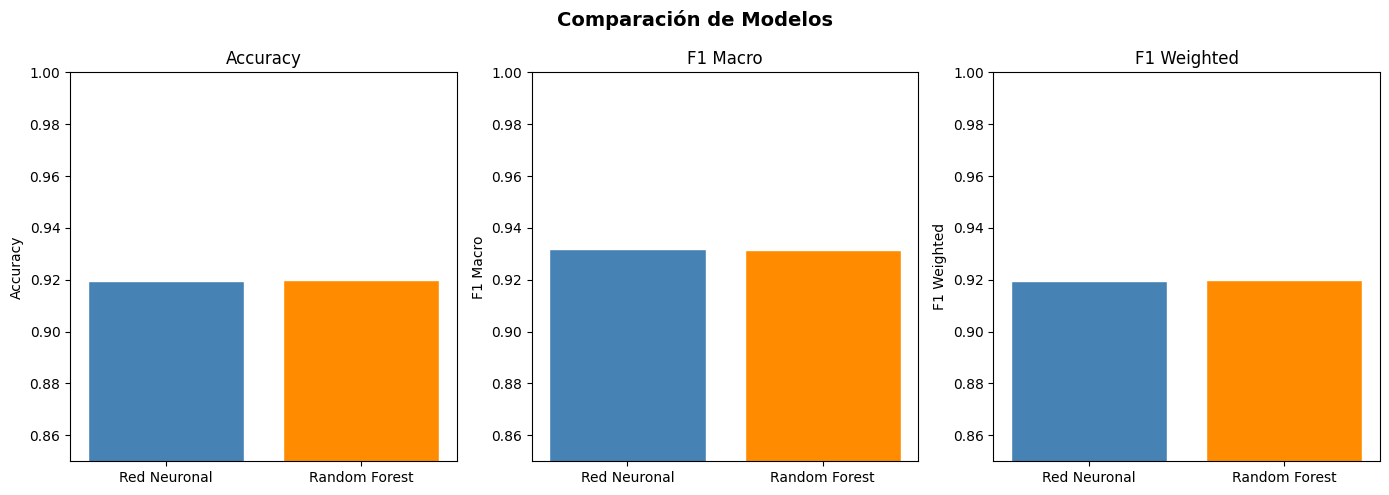
\includegraphics[width=\textwidth]{comparacion_clasificacion.png}
    \caption{Comparación de los modelos de clasificación.}
    \label{fig:comparacion_clasificacion}
\end{figure}

\subsection*{4. Discusión y conclusiones}

Ambos modelos presentan un rendimiento muy alto en la clasificación de variedades de 
judía, con accuracies superiores al 91\% y F1-scores en torno a 0.93. Las diferencias 
entre la red neuronal y el Random Forest son mínimas, por lo que ambos modelos pueden 
considerarse prácticamente equivalentes en este problema.

A nivel de clases, Bombay es clasificada perfectamente por ambos modelos, lo 
que confirma su clara separabilidad en el espacio de características. En contraste, 
Sira es la clase más compleja, debido a su solapamiento con Dermason
y Cali, lo que reduce su F1-score.

Para mejorar el rendimiento de la red neuronal, se podrían aplicar técnicas como 
Early Stopping para evitar sobreajuste, así como explorar arquitecturas más 
profundas y un mayor número de épocas de entrenamiento.

\end{document}